\documentclass{standalone}
\usepackage{tikz}
\usetikzlibrary{matrix, positioning,calc,arrows.meta, backgrounds,fit}
\usepackage[dvipsnames]{xcolor}
\usetikzlibrary{shapes.geometric}
\tikzset{
    every node/.style={font=\small},
    rectred/.style={draw=red, fill=green!80!black!10, thick, rounded corners,  align=center},
    rectblue/.style={draw=blue,  rounded corners, align=center},
    yellowbox/.style={draw=black, fill=Dandelion, thick, rounded corners, align=center},
    greencycle/.style={fill=green!80!black!10,ellipse, align=center},
    bluecycle/.style={fill=NavyBlue, ellipse, align=center},
    arrow/.style={-{Latex[length=3mm]}, thick},
}
\begin{document}
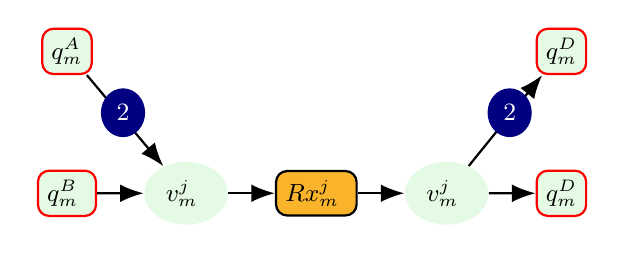
\begin{tikzpicture}[node distance=12mm and 0mm]
% Define the row width (distance between start and end nodes)
\def\rowwidth{60mm}
\def\sep{6mm}
\def\sepp{12mm}
% width of the side bands (change as you like)
\matrix (top) [matrix of nodes,column sep=\sep] {
  |[rectred]| $q_m^{B}$ & |[greencycle]| $v_m^{j}$ & |[yellowbox]| $Rx_m^{j}$ & |[greencycle]| $v_m^{j}$ & |[rectred]| $q_m^{D}$\\  
};
\node[rectred,above=\sepp of top-1-1] (A)  {$q_m^{A}$} ;
\node[rectred,above=\sepp of top-1-5] (D)  {$q_m^{D}$} ;
\foreach \i in {1,...,4}{
  \pgfmathtruncatemacro{\j}{\i+1} % compute i+1 as integer
  \draw[arrow] (top-1-\i) -- (top-1-\j);
}
\draw[arrow] (A) -- (top-1-2);
\node[bluecycle,above= 3mm of top-1-2,xshift=-8mm] (z1)   {\textcolor{white}{$2$}} ;
\draw[arrow] (top-1-4) -- (D);
\node[bluecycle,above= 3mm of top-1-4,xshift=8mm] (z2)   {\textcolor{white}{$2$}} ;
\end{tikzpicture}
\end{document}
